% =============================================================================
%  Script Fragility in Sinhala
%  ACL submission, anonymous review version.
%
%  COMPILER: pdfLaTeX.
% =============================================================================
\documentclass[11pt]{article}
\usepackage[review]{acl}

% ---- fonts and encodings -----------------------------------------------------
\usepackage{times}
\usepackage{latexsym}
\usepackage[T1]{fontenc}
\usepackage[utf8]{inputenc}
\usepackage{microtype}
\usepackage{inconsolata}

\usepackage[safe]{tipa}

\usepackage{graphicx}
\usepackage{booktabs}
\usepackage{amsmath}
\usepackage{amssymb}
\usepackage{multirow}
\usepackage{array}
\usepackage[normalem]{ulem}

\usepackage{subcaption}
\captionsetup[sub]{font=small,labelfont=bf,skip=3pt}
\captionsetup{subrefformat=parens}   % \subref prints "(a)", as the panel does

% ---- Sinhala examples --------------------------------------------------------
\makeatletter
\newcommand{\sinhalaglyph}[1]{%
  \raisebox{-0.25\height}{%
    \includegraphics[height=1.2\dimexpr\f@size pt\relax]{sinhala/#1}}}
\makeatother

\newcommand{\siex}[2]{\sinhalaglyph{#1}\,[\textipa{#2}]}


\newcommand{\sikohomada}{\siex{si-kohomada}{k6h6m2D2}}      % kohomada
\newcommand{\sitha}{\siex{si-tha}{T2}}                      % th
\newcommand{\siwa}{\siex{si-wa}{v2}}                        % w
\newcommand{\siwesak}{%                                       % wesak
  \sinhalaglyph{si-wesak}%
  \space\sinhalaglyph{si-uthsawayeedii}%                      % uthsawayeedii
  \space\siex{si-bauddhayin}{vEs2k UTs2v2je:Di: baUDD\super{h}2jIn}}% bauddhayin
\newcommand{\sinya}{\siex{si-nya}{\textltailn 2}}           % the nya sequences
\newcommand{\sika}{\siex{si-ka}{k2}}                        % ka, inherent vowel
\newcommand{\sikaa}{\siex{si-kaa}{ka:}}                     % kaa, vowel sign
\newcommand{\sikhal}{\siex{si-khal}{k}}                     % k, hal kirima
\newcommand{\sisinhala}{\siex{si-sinhala}{sI\ng h2l2}}      % the language name

% ---- helpers -----------------------------------------------------------------
\newcommand{\rom}[1]{\textit{#1}}                 % Romanized Sinhala
\newcommand{\bpb}{\textsc{bpb}}
\newcommand{\bpw}{\textsc{bpw}}
\newcommand{\bpc}{\textsc{bpc}}
\newcommand{\mcc}{\textsc{mcc}}

% Float placement. 
\setcounter{topnumber}{3}
\setcounter{bottomnumber}{2}
\setcounter{totalnumber}{5}
\renewcommand{\topfraction}{0.92}
\renewcommand{\bottomfraction}{0.6}
\renewcommand{\textfraction}{0.06}
\renewcommand{\floatpagefraction}{0.72}
\renewcommand{\dbltopfraction}{0.92}
\renewcommand{\dblfloatpagefraction}{0.72}
\setcounter{dbltopnumber}{3}

\usepackage{ifthen}
\usepackage{todonotes}
\newboolean{reviewmode}
\setboolean{reviewmode}{true}   % ← flip to false to hide all notes

\definecolor{ndscolor}{HTML}{fb1010}
\newcommand{\nds}[1]{\ifthenelse{\boolean{reviewmode}}{\textcolor{ndscolor}{$_{nds}$[\textbf{#1}]}}{}}
\newcommand{\ndstodo}[1]{\ifthenelse{\boolean{reviewmode}}{\todo[color=ndscolor]{$_{nds}$ {\footnotesize #1}}}{}}

\definecolor{studentcolor}{HTML}{ca5800}
\newcommand{\stu}[1]{\ifthenelse{\boolean{reviewmode}}{\textcolor{studentcolor}{$_{students}$[#1]}}{}}
\newcommand{\stutodo}[1]{\ifthenelse{\boolean{reviewmode}}{\todo[color=studentcolor]{$_{Students}$ {\footnotesize #1}}}{}}
\makeatletter
\newcommand{\rows}[1]{\@@input #1 }
\makeatother

% Anonymous placeholder. Replace before camera-ready. The transliterator is on
% PyPI, but naming the package would identify us, so the name is withheld until
% the camera-ready version.
\newcommand{\anonrepo}{\url{https://anonymous.4open.science/r/sinhala-script-robustness-llm}\nds{Great that you are giving this here. But you need to go though it and make sure there are no names or references to us. For example, I found my name in a folder.}\stu{Corrected it sir.}}

\title{Script Fragility in Sinhala: Tokenizer-Independent and Downstream\\
Evidence from Small Language Models}

\author{Anonymous ACL submission}

% No widow or orphan lines, asked for in review.
\widowpenalty=10000
\clubpenalty=10000

\begin{document}
\maketitle

\begin{abstract}
Sinhala is written online in two ways. Formal text uses the Sinhala script, while
comments, chat and social media are written in Romanized Sinhala, in Latin
letters\nds{The types should precede the listing or it looks like types are only relevant to latter}\stu{fixed it sir}. A
recent benchmark reported that language models are roughly 312 times worse on
Romanized than on Sinhala-script text, and that parameter count predicts ability in
neither script. Both results rest on perplexity, which is normalized by token count
and not comparable across tokenizers. We remeasure 31 small open-weight
checkpoints (350M to 14.7B) with bits per byte, matching the published perplexities to a
median of 0.05\%\nds{exactly?}\stu{Not exactly sir, and we have replaced the word and added the difference. Appendix~\ref{sec:repro24}
now says it clearly and Table~\ref{tab:shared24} lists every comparison.}, so what changes is the metric. The reported
ratio then splits in two on the same 24 checkpoints, a factor of 21 from identical
content being cut into a different number of tokens and a factor of 24 from a real
rise in per-byte loss. Under bits per byte, parameter count is associated with
Sinhala-script ability. The clearest case is SinLlama, a Sinhala-adapted Llama-3-8B,
which reports the smallest degradation of any checkpoint here, 8.7-fold, and one of the
largest real per-byte gaps. We then report the first downstream evaluation of Sinhala
script variation using 9{,}479
items, three tasks, eleven instruction-tuned checkpoints, 208{,}538 generations. A 22.4
point spread in Sinhala-script accuracy narrows to 6.7 under romanization, and Romanized
accuracy rises with Sinhala-script accuracy at a slope of 0.22 (95\% CI 0.11 to 0.54). On
offensive-language detection, accuracy moves by a few points while Matthews correlation
loses over half its value. Longer input does not explain this difference because these tokenizers fall back to byte-level pieces when processing Sinhala script, resulting in less efficient tokenization, so the Romanized prompt is the \emph{shorter} of the two in tokens
for every checkpoint\nds{What? How?}\stu{Sir most of these tokenizers have no
Sinhala pieces and fall back to byte level, which generate more tokens per Sinhala
word than the same word romanized. So romanizing makes the prompt
shorter. This is now stated in the
abstract and measured per checkpoint in Table~\ref{tab:invalidtau}.}. Absolute Sinhala-script bits per byte tracks the size of
that gap but the bits-per-byte \emph{gap} does not.
\end{abstract}

% =============================================================================
\section{Introduction}
\label{sec:intro}

Sinhala is an Indo-Aryan language with a script of its own, spoken by over 17 million
people, almost all in Sri Lanka \citep{desilva-2019-survey,
ranasinghe-etal-2025-sold}. Like several South Asian languages it has an everyday
orthographic split: formal writing uses the Sinhala script, but comments, chat and
social media are dominated by Romanized Sinhala, informally called \textit{Singlish}
in Sri Lanka,\footnote{The same word is used for Colloquial Singapore English, which
is unrelated. Throughout this paper \textit{Singlish} means Romanized Sinhala, the
sense it carries in Sri Lanka.}\nds{Will need to disclaim against Singapore English}\stu{Added as a footnote sir} typed
with Latin letters. It has no standard spelling, so \sikohomada{} (``how are you'')
is typed \rom{kohomada}, \rom{kohomd} or \rom{kohomade} depending on the writer.
A deployed Sinhala system therefore serves mostly Romanized input while being
evaluated on Sinhala-script benchmarks (\S\ref{sec:related}).

\citet{rajapakse-weerasinghe-2026-script} gave the first systematic measurement
for Sinhala. Benchmarking 24 open weight models with perplexity, they reported a
median 312-fold degradation from Sinhala-script to Romanized text and no
correlation between parameter count and script handling. Both findings rest on a
metric that is not comparable across models.\nds{Need to add a space after the full stop. I am only mentioning it here. But fix it everywhere}\stu{Fixed sir} Perplexity is normalized by token count,
and token count depends on the tokenizer\nds{Did you look at the tokenisers by~\citet{ekanayake2026helabert}, \citet{aravinda2025sinllama}, \citet{velayuthan-sarveswaran-2025-egalitarian}, and \citet{nisfer2026grapheme}?}\stu{We had not sir. We looked into these papers and it was a real gap. All four are now
discussed in \S\ref{sec:related} and also we measured them sir (Appendix~\ref{sec:tokenizers}). The results on our own corpus are as below.
HelaBERT 1.31 and
SinLlama 1.44 tokens per Sinhala word, against 4.34 to 14.20 across our 31 general
checkpoints. So a Sinhala vocabulary cuts Sinhala script fertility by three to seven
times. What it does not do is help the Romanized register, where SinBERT is the worst
of every tokenizer we tried at 6.15 tokens per word. That is the sharpest evidence we
have for the paper's argument. Thank you sir for pointing us at it. We also took the
SinLlama model itself the whole way through the intrinsic protocol
(\S\ref{sec:sinllama}).}, which for Sinhala varies by more than a
factor of three. They also note that perplexity says nothing about whether a model can
still do anything useful, and call for downstream evaluation. We take up both
problems.

We recompute bits per byte for 31 small open-weight checkpoints over the same
parallel corpus (\S\ref{sec:intrinsic}). Our perplexities reproduce the published
values to a median of 0.05\%, so what changes below is the metric. Across the pool,
perplexity and bits per byte are unrelated ($\rho = 0.08$) while perplexity is almost
fully explained by tokenizer fertility ($\rho = -0.87$), and the reported ratio
splits into a factor of 21 from token-count normalization and 24 from a real rise in
per-byte loss. Under bits per byte, parameter count does predict
Sinhala-script ability ($\rho = -0.55$), though not Romanized ability. We then score
SinLlama \citep{aravinda2025sinllama}, a Sinhala-adapted Llama-3-8B, against the exact
checkpoint it was built from (\S\ref{sec:sinllama}). It is the case where the two
metrics disagree most. The adaptation halves its cost per byte on the Sinhala script
and multiplies its perplexity by 23.

We then evaluate eleven instruction-tuned checkpoints on 9{,}479 items in both
scripts (\S\ref{sec:extrinsic}). Romanization narrows a
22.4 point spread in Sinhala-script accuracy to 6.7 points, so most of a checkpoint's
advantage does not carry over. Absolute Sinhala-script bits per byte
tracks that gap ($\rho = -0.83$); the reported bits-per-byte \emph{gap} does not. Building the Romanized side needed a Sinhala-to-Latin transliterator, released
as a pip package.


% =============================================================================
\section{Related Work}
\label{sec:related}

\paragraph{Sinhala and low resource evaluation.}
Sinhala is low resource and its tooling has grown in a fragmented way
\citep{desilva-2019-survey, ranathunga-de-silva-2022-languages, joshi-etal-2020-state}.
Recent resources are almost entirely Sinhala-script like SinhalaMMLU
\citep{pramodya-etal-2025-sinhalammlu}, SOLD \citep{ranasinghe-etal-2025-sold}, the
Sinhala split of Global PIQA \citep{desilva-ranathunga-2026-sinhalapiqa,
chang-etal-2025-globalpiqa} and encoder work such as
\citet{dhananjaya-etal-2022-bertifying}. Each uses a single orthography, so a model can be
evaluated on all of them without being tested on the register most of its users write in.
The only benchmark treating script as a variable is
\citet{rajapakse-weerasinghe-2026-script}, which we extend.

\paragraph{Romanized registers in deployment.}
Romanized writing is not a marginal input condition. Code-mixed and Romanized registers
persist for durable social and economic reasons rather than fashion
\citep{sengupta-etal-2024-hinglish}, and they dominate real traffic.
\citet{khullar-etal-2025-scriptgap} found 83\% of Hindi and 73\% of Telugu messages
Romanized in a maternal-health service handling live queries, with weighted F1 falling by
as much as 24 points when those queries arrive in Latin script. That is the closest
existing result to ours. Romanized Sinhala adds the difficulty of having no orthographic
standard at all, averaging 15.7 accepted Romanized spellings per word in the Swa-bhasha
lexicon \citep{sumanathilaka-etal-2025-swabhasha}.

\paragraph{Romanization in other languages.}
Romanized South Asian text has been studied mainly as a resource and identification
problem \citep{roark-etal-2020-processing, benton-etal-2025-improving}. \citet{husain-etal-2024-romansetu}\nds{check ref}\stu{Checked it and fixed it sir. We corrected the entry and it now reads ``Husain et
al.''.} show romanization can \emph{help} once a model is
adapted for it, the mirror image of the zero-shot setting we study. Work on Sinhala trains
models for the register rather than measuring general ones
\citep{chamikara-sumanathilaka-2026, hewapathirana-sumanathilaka-2024-emoscan}, and
transliteration tooling points from Latin into Sinhala rather than out of it
\citep{de-mel-etal-2025-sinhala, sumanathilaka-etal-2025-swabhasha}. We ask instead what
general-purpose generative models do out of the box, with a paired item-level design, a
competence screen, and a test of whether the gap is a tokenization artifact.

\paragraph{Tokenizer-independent evaluation.}
Perplexity is normalized by the number of tokens a model's own vocabulary produces,
so two models that assign the same probability to the same string can report
different perplexities. Bits per byte was introduced to remove that dependence
\citep{gao-etal-2020-pile}, and the language-modeling benchmark PALOMA\nds{Who this?}\stu{Named properly now. It is a language modelling benchmark and we cite it because it adopts bits per byte for reason we do.
}, from the
Allen Institute for AI, adopts it for cross-model comparison for the
same reason \citep{magnusson-etal-2024-paloma}. The problem is the sharpest for scripts
that tokenizers serve unevenly \citep{petrov-etal-2023-tokenizers,
ahia-etal-2023-languages}, and over-segmentation carries a measurable downstream
cost on low resource tasks \citep{nag-etal-2024-fragmented}. Sinhala sits at that
extreme, with fertility on our corpus ranging from 4.3 to 14.2 tokens per word.
Bits per byte is established practice in language modeling, but to our knowledge
it has not previously been used to show that the substantive conclusions of a
published multilingual benchmark change when the normalizer changes.

\paragraph{Sinhala tokenizers.}
Since fertility is most of what perplexity on Sinhala reflects, tokenizer work for the
language matters here. \citet{velayuthan-sarveswaran-2025-egalitarian} argue that unequal
representation between languages starts with the tokenizer, and
\citet{nisfer2026grapheme} give grapheme level tooling for scripts where one written
unit spans several code points. HelaBERT \citep{ekanayake2026helabert} and SinLlama
\citep{aravinda2025sinllama} train Sinhala vocabularies, which cut Sinhala-script
fertility to 1.3 and 1.4 tokens per word against 4.3 to 14.2 across our pool. Neither
helps the Romanized register, and the Sinhala only vocabulary of SinBERT
\citep{dhananjaya-etal-2022-bertifying} is the least efficient on it of any tokenizer we
measured (Appendix~\ref{sec:tokenizers}). This work fixes the Sinhala-script side and
leaves the register most users write in where it was.

% =============================================================================
\section{Experimental Setup}
\label{sec:setup}

\nds{Some people (eg: my PhD supervisor), do not like when topics are stacked like this with no text.}\stu{Fixed here and in section 4. Both sections now start with a small paragraph that says what the section does.
}

Our entire setup follows one rule. The script is the only thing that changes between the two test conditions. This requirement guides how we set up the data, models, prompts, and statistical tests, which are covered in the subsections below. Appendix~\ref{sec:sinhala} provides background on Sinhala and its writing system.

\subsection{Script conditions and data}

Every item is evaluated twice, once in the Sinhala script as published and once
romanized with identical content, so all comparisons are paired and differ only in
orthography. Both conditions come from the Sinhala-script source through our own transliterator,
including for Global PIQA, which also publishes a Latin-script config that
\S\ref{sec:licenses} explains we do not use. The intrinsic corpus is the parallel set
released with \citet{rajapakse-weerasinghe-2026-script}, which contains 500 sentence pairs whose
Romanized side native speakers typed, so the intrinsic results do not depend on our
transliterator. A separate 500-sentence mixed-script corpus supports a secondary
condition.

Downstream we use every available item with no sampling. SinhalaMMLU is a
6{,}879-item curriculum-aligned multiple-choice benchmark in the style of MMLU
\citep{hendrycks-etal-2021-mmlu}, over six domains and three difficulty levels, and 2{,}145
of its items have five options rather than four, so guessing scores 23.4\%.\footnote{The public Hugging Face
release contains a 1{,}851-item sample. We obtained the full set from the
authors, who ask that it not be redistributed, so we release our transformation
code and item identifiers rather than the items
(\S\ref{sec:licenses}).\nds{We can release the transformations of the public 1851, can't we?}\stu{Sir SinhalaMMLU is CC BY-NC-ND, and the NoDerivatives term forbids distributing adapted material regardless of which subset it came from. Our Romanized version is an adaptation, so the public 1,851 items are blocked for the same reason as the full set}} SOLD supplies the complete 2{,}500-item test split of a
binary offensive-language task in which 40.6\% of posts are offensive, so the majority
class scores 59.4\%. Global PIQA, which follows PIQA \citep{bisk-etal-2020-piqa},
contributes the 100 Sinhala items of its released non-parallel split.
\citet{desilva-ranathunga-2026-sinhalapiqa} wrote and cross-verified 110, of which 77 of
the released 100 carry \texttt{approx\_cultural\_score}${}=1$\nds{where did you get this number 77 from?}\stu{We got that number from the dataset's metadata file sir. Not from the paper. 
In the dataset exactly 77 items have the tag approx\_cultural\_score = 1. We updated the text to explicitly name this metadata field too.}. Together the three sets give
9{,}479 items, or 18{,}958 prompts per checkpoint.

\subsection{Building the Romanized data}
\label{sec:translit}

Almost every Sinhala transliteration tool runs Latin to Sinhala rather than the reverse
(\S\ref{sec:related}), so we implemented a deterministic grapheme-level transliterator
that parses Sinhala as an abugida and uses the digraph conventions speakers commonly type,
so \sitha{} is \rom{th} and \siwa{} is \rom{w}. It runs locally, covers every input, and
collapses only the consonant distinctions casual Singlish also collapses, turning
\siwesak{} into \rom{wesak uthsawayeedii bauddhayin}.

We validated it against 755{,}000 human-romanized items from the Swa-bhasha
Resource Hub \citep{sumanathilaka-etal-2025-swabhasha}, which contains 4{,}397 authentic
social-media sentence pairs, 450{,}587 words each carrying several accepted
spellings, and a 300{,}000-sentence machine-augmented cross-check. Scored against
the closest accepted reference by character error rate, chrF
\citep{popovic-2015-chrf} and exact match, ours has the lowest error rate of the four
methods on all three corpora, 0.182, 0.121 and 0.112, and a paired Wilcoxon test
separates it from Aksharamukha \citep{rajan-aksharamukha}, uroman
\citep{hermjakob-etal-2018-box} and the web romanizer released for
\citet{desilva-ranathunga-2026-sinhalapiqa} at $p < 0.001$ on both large corpora.

What is left is convention rather than phonemic error, chiefly that all four methods
double long vowels far more often than people do, 0.81 per word against 0.12. Word by
word against the human-typed side of the parallel corpus, 44.6\% of our forms match
exactly and a further 27.6\% once that convention is normalized against the
multi-reference lexicon, 88.6\% of our spellings are ones a human supplied for that
word, against 84.2\% for the native speakers who typed the same sentences.
Appendix~\ref{sec:translitdetail} gives the comparison, and \S\ref{sec:translitbias}
shows the residual makes our Romanized condition harder rather than easier.

\subsection{Models}

The intrinsic evaluation covers 31 decoder-only checkpoints from 350M to 14.7B
parameters, all within the range usually described as small language models, and
spanning the Llama \citep{grattafiori-etal-2024-llama3}\nds{You are using Llama-3.1-8B then  you need to test against SinLlama~\cite{aravinda2025sinllama} which is based on Llama-3-8B}\stu{Done sir, and it turned out to be the most useful measurement in
the paper. We scored SinLlama and, because it is built on Llama-3-8B, we also scored Meta-Llama-3-8B, so
the comparison isolates the Sinhala adaptation. \S\ref{sec:sinllama} and Table~\ref{tab:sinllama} report it}, Qwen
\citep{yang-etal-2024-qwen2, yang-etal-2025-qwen3}, Gemma
\citep{gemmateam-2024-gemma2}, Mistral, BLOOM \citep{lescao-etal-2023-bloom}, OPT,
Pythia \citep{biderman-etal-2023-pythia} and Phi \citep{abdin-etal-2024-phi4}
families. Twenty-four are exactly the pool
\citet{rajapakse-weerasinghe-2026-script} used, plus three newer base checkpoints and
four instruction-tuned counterparts (Appendix Table~\ref{tab:modelids}). Downstream needs
models that follow a response format, so it uses the eleven instruction-tuned
checkpoints, from 1.1B to 14.7B; two cannot follow it at all in the Sinhala-script
condition, which \S\ref{sec:screen} handles explicitly rather than by dropping them.

\subsection{Prompting and scoring}
\label{sec:prompting}

All downstream prompts are zero-shot and greedily decoded with a 40-token limit.
We picked one template from three candidates using a pilot of 3{,}240 generations over
nine checkpoints, both scripts and 20 items per dataset. The direct template won on
SinhalaMMLU, the largest set, and was the only candidate that never produced an
unparseable answer there. An answer-first template scored 1.4 points higher on SOLD and
7.2 higher on Global PIQA. We used the direct template everywhere regardless, because
choosing per dataset would confound task with prompt and because 20 items cannot resolve
differences of that size. A paired comparison needs a template that does not favor a
script rather than an optimal one, and the evidence for that comes from the main run,
where the unparseable rate never exceeds 0.03\% in either condition for the competent
cohort (\S\ref{sec:controls}). Answers are extracted by pattern match and anything
unparseable is scored wrong. Twenty pilot items, 0.3\% of SinhalaMMLU, also appear in the
evaluation set. All three templates are in Appendix~\ref{sec:prompts}.

\subsection{Significance testing}
\label{sec:stats}

Both conditions score the same items, so we use McNemar's continuity-corrected test
\citep{mcnemar-1947, dror-etal-2018-hitchhikers} and report the discordant pair counts,
controlling the family-wise error rate over checkpoints within each dataset with Holm's
procedure \citep{holm-1979}. Intervals on gaps, macro-F1 and Matthews correlation
differences and regression slopes come from 10{,}000 paired bootstrap resamples. For SOLD
we lead with Matthews correlation \citep{matthews-1975, chicco-jurman-2020}, since the
classes are imbalanced and accuracy sits close to the majority baseline. Item-level
effects are also fitted as logistic regressions with checkpoint fixed effects and
item-clustered standard errors.

\subsection{The competence screen}
\label{sec:screen}

Some checkpoints score at the guessing baseline even in the Sinhala script. For those,
romanization cannot make the score drop much, because there is no skill left to lose,
so their small gap is not evidence that they handle Romanized text well\nds{No idea what the sentence up to this point means}\stu{Rewritten sir. The point we were trying to make is that a model already at the guessing baseline in the Sinhala script cannot show a drop when the script changes, because it has nothing left to lose, so counting its zero gap in an average pulls the average down for the wrong
reason. That is why we screen on Sinhala-script competence first}. Averaging
such a gap in with the rest pulls the group mean towards zero. We mark a checkpoint
\emph{competent} on a task when its Sinhala-script score beats the guessing
baseline at $p < 0.01$ under a Poisson-binomial null and it does not put more than
90\% of its answers on one option. Six of eleven pass on SinhalaMMLU, six have a
non-trivial signal on SOLD, and none pass on Global PIQA. All eleven appear in
every table. Absolute performance is low throughout, as it tends to be for small open
checkpoints on a low resource language. However the best Sinhala-script score on SinhalaMMLU is
44.1\% against a 23.4\% baseline. What we test is the paired difference within a
checkpoint\nds{So as a whole not great results on any?}\stu{Actually yes sir. The overall scores are low. As we see SMLs struggle with Sinhala out of the box, and Global PIQA is a very tough benchmark for them because it tests local cultural knowledge too. Our goal is not to get high benchmark scores, but to measure how much a model drops when switching from Sinhala letters to Singlish. The test filter simply makes sure a model can do the task in Sinhala first, so we do not mistake a model that is just guessing for one that handles both scripts well.}, not its standing against
other models.


% =============================================================================
\section{Re-measuring the Intrinsic Gap}
\label{sec:intrinsic}

This section re-runs the measurement of \citet{rajapakse-weerasinghe-2026-script} with
the token count out of the denominator. We state the metric, check that our forward
passes reproduce their perplexities, and only then change the normalizer, so any
difference in conclusions comes from the metric and not from a different run.

\subsection{Tokenizer-independent metrics}

For a text $s$ we accumulate the model's total negative log-likelihood
$\mathrm{NLL}(s)$ in nats and divide by a unit of the text itself rather than by
its tokenization:
\begin{equation}
\bpb = \frac{\sum_s \mathrm{NLL}(s)}{\ln 2 \sum_s |s|_{\text{bytes}}},
\label{eq:bpb}
\end{equation}
and likewise per character (\bpc) and per whitespace word (\bpw). The denominator no
longer depends on the tokenizer. The numerator still does, since a model's loss reflects
how its own vocabulary carves up the string, so Equation~\ref{eq:bpb} removes the
arbitrary unit of account rather than every trace of tokenization. We pool numerator and
denominator over the corpus instead of averaging per-sentence ratios, so short sentences
do not dominate. Bytes are the standard choice \citep{gao-etal-2020-pile}, but \bpw{} is
the sharpest across scripts, because a sentence and its romanization have the same word
count while Sinhala UTF-8 spends 2.65 bytes per character against 1.00 for Latin.

Our recomputed perplexities reproduce the published values for all 24 shared
checkpoints, with median absolute deviation 0.05\% on Sinhala-script and 0.004\% on
Romanized text, and 0.39\% on mixed script once two outliers are excluded. Appendix
Table~\ref{tab:shared24} sets our recomputation beside every headline number of the
original benchmark, so everything below reflects the metric and not a different
run.

\subsection{Perplexity tracks tokenizer fertility}

Across the 31 checkpoints, Sinhala-script perplexity and Sinhala-script bits per byte
are statistically unrelated ($\rho = 0.08$, $p = 0.68$), as are the Romanized values
($\rho = 0.13$, $p = 0.48$). Only one of the five best by perplexity is among the five
best by bits per byte. Gemma-2-9B ranks 26th of 31 on perplexity and 2nd on bits per
byte, and Qwen3.5-9B-Base moves from 28th to 6th.

The cause is visible in Figure~\ref{fig:ppl-fert}. Perplexity is almost fully explained
by how many tokens a tokenizer spends on a Sinhala word ($\rho = -0.87$, $p < 10^{-9}$),
which ranges from 4.3 for the Qwen3.5 and Gemma tokenizers to 14.2 for models that fall
back to bytes. Spreading the same loss over three times as many tokens lowers per-token
perplexity without the model knowing anything more, so comparing perplexity across
families on Sinhala is largely comparing tokenizers. How far the two come apart depends
on the pool. On the 24 checkpoints of \citet{rajapakse-weerasinghe-2026-script} the rank
correlation is moderate ($\rho = 0.46$, $p = 0.02$), still leaving four fifths of
bits-per-byte rank variance unexplained, and adding the seven newer checkpoints removes
even that. The disagreement is not an artifact of our additions, but it grows as modern
tokenizers enter the comparison.

\subsection{Decomposing the reported ratio}
\label{sec:decomp}

The degradation ratio can be decomposed exactly. Since
perplexity is $\exp(\mathrm{NLL}/T)$ for $T$ scored tokens and
$\mathrm{NLL} = \ln 2 \cdot A \cdot B$ for $A$ bits per byte over $B$ bytes,
\begin{equation}
\log_2 \mathrm{PPL} = A \cdot x, \qquad x = B/T,
\label{eq:identity}
\end{equation}
where $x$ is the bytes each token carries. Across the two script conditions the
change in $\log_2 \mathrm{PPL}$ is then exactly
\begin{equation}
\underbrace{\bar{A}\,(x_r - x_u)}_{\text{token-count normalizer}}
+ \underbrace{\bar{x}\,(A_r - A_u)}_{\text{per-byte loss}},
\label{eq:decomp}
\end{equation}
with $\bar{A}$ and $\bar{x}$ the two-condition means. The first term is the part of the
reported degradation caused by identical content being cut into a different number of
tokens, the second the part caused by the model assigning less probability per byte. The
split is an exact algebraic identity, not an empirical model.

On the 24 checkpoints of \citet{rajapakse-weerasinghe-2026-script}\nds{what is this prior work? refer explicitly}\stu{Fixed sir. There were seven “Prior work” references. Added the correct citation to
\citet{rajapakse-weerasinghe-2026-script}.} the median gap is 8.29 bits, which is the 312-fold
ratio they report. Equation~\ref{eq:decomp} assigns 4.37 bits to the normalizer and 4.56 to per-byte loss,
factors of 21 and 24 whose product is the published 312, so almost exactly half the
reported degradation is the unit of account. Over all 31 checkpoints the normalizer share
falls to 39\%, and for the six Qwen3.5 and Gemma checkpoints it is slightly negative
(Appendix Table~\ref{tab:decomp}). Those six also report the five smallest ratios, with
the four Qwen3.5 entries between 58-fold and 64-fold against a pool median of 294-fold,
so the largest reported ratios come from the models whose tokenizers handle Sinhala
worst.

\nds{This paragraph is too obvious that it is AI written. I mean the whole paper is. But this paragraph is way too obvious}\stu{Rewritten sir.}This matters in two ways. The ratio makes the models look worse on Romanized
Sinhala than they are. Measured per byte the same gap is 2.14 bits, which is a factor
of 4.4, and per word it is 1.11 bits. It also removes the basis for the claim that
scale does not help. Parameter count is uncorrelated with Sinhala-script perplexity
($\rho = 0.15$, $p = 0.42$), but it is correlated with Sinhala-script bits per byte
($\rho = -0.55$, $p = 0.001$) and with mixed-script bits per byte ($\rho = -0.57$,
$p = 0.0008$), and that holds on the 24 checkpoints of
\citet{rajapakse-weerasinghe-2026-script} on their own ($\rho = -0.42$, $p = 0.04$).
Romanized ability stays uncorrelated with scale ($\rho = -0.28$, $p = 0.13$). We would
not call this a scaling result, because the checkpoints differ in family, tokenizer and
training corpus at the same time. It is an association across models.


\subsection{Romanization narrows the spread}

Figure~\ref{fig:flat-lm}\nds{Use subfig or sub-caption and directly refer. Do not hard code}\stu{Done sir. We now create a separate PDF for each panel and use LaTeX subfigures. Nothing is typed manually.}
 shows the effect that the rest of the paper examines.
Sinhala-script cost spans 16.3 to 34.1 bits per word, a spread of 17.7 bits, while
Romanized cost spans 20.3 to 25.7, a spread of 5.4. Regressing one on the other, a full
bit per word of Sinhala-script improvement buys only 0.14 bits on Romanized text (95\% CI
0.05 to 0.25, $R^2 = 0.19$). Twelve of the 31 checkpoints are cheaper on Romanized text,
and which ones is predictable. The better a checkpoint is on the Sinhala script, the more
it loses ($\rho = -0.88$, $p < 10^{-9}$). The mixed-script condition behaves differently
and reproduces the earlier finding, with Sinhala-script and mixed bits per byte
rank-correlated at $\rho = 0.94$ and a median gap of 0.49 bits, against $\rho = 0.41$ for
Romanized. Interleaving the two scripts is a mild perturbation; replacing one is not.

\subsection{A Sinhala-adapted checkpoint}
\label{sec:sinllama}

Every checkpoint above was built without Sinhala in mind, so the disagreement between the
metrics could be an artifact of tokenizers never meant to carry the script. SinLlama \citep{aravinda2025sinllama} tests this approach. It uses Llama-3-8B with 11{,}080 Sinhala pieces merged
into its vocabulary and continual pre-training on 10.7M Sinhala sentences. We scored it and
Llama-3-8B itself, so the two rows of Table~\ref{tab:sinllama} differ only by the
adaptation.

The adaptation works and bits per byte says so, with Sinhala-script cost falling from
1.157 to 0.628, the lowest of the 32 checkpoints. Perplexity rises from 3.25 to 74.56,
the highest of the 32, because the tokenizer stopped spending 9.68 tokens on a Sinhala
word and started spending 1.44. What matters here is the reported degradation ratio,
which falls from 311 to 8.7, by far the smallest in the pool, while the real per-byte gap
widens from 2.447 to 2.743 bits, exceeded by only one of the 31. The adaptation bought
0.528 bits per byte on the Sinhala script and 0.233 on Romanized text, favoring the formal alphabet over how most people actually type. The standard published metric falsely makes it look like the most balanced model, but the bits per byte metric proves that it is one of the worst (Appendix~\ref{sec:sinllamadetail}).

\subsection{Comparison with $n$-gram models}

Relative comparisons leave open whether these models are merely worse on Romanized text
or close to uninformed about it, so we fit add-1 character $n$-gram references on the
same corpus under five-fold cross-validation. On Romanized Sinhala the best $n$-gram
reaches 2.64 bits per byte and a character bigram 3.06, while the best of the 31
checkpoints reaches 3.29 and the median 3.81, so none beats the bigram. On the Sinhala
script the ordering is the expected one, with the character trigram at 1.16 and one
checkpoint below it (Appendix Table~\ref{tab:ngram}). An in-domain $n$-gram is a cheap
model and the comparison favors it, so we read this as the checkpoints failing to use
Romanized structure beyond what a character bigram captures, not as a claim about what
they know.


% =============================================================================
\section{Downstream Consequences}
\label{sec:extrinsic}

Table~\ref{tab:main} reports every checkpoint on SinhalaMMLU and SOLD. Global PIQA is in Appendix Table~\ref{tab:piqa}, since at 100 items it supports a much
coarser comparison than the other two, and \S\ref{sec:piqa} discusses it\nds{no PIQA because all failed?}\stu{Now all 11 models are fully reported on Global PIQA in Table~\ref{tab:piqa}. In Section~\ref{sec:piqa}, we now included why 100 items is small to resolve a performance gap sir. We also re-ran it with the corrected prompt.}.

\subsection{Multiple-choice knowledge}

Four of the six competent checkpoints lose significantly under romanization after Holm
correction. Qwen3.5-9B falls from 44.1\% to 28.7\%, a 15.5 point drop (95\% CI 14.0 to
16.9, 1{,}892 against 828 discordant pairs), Qwen3.5-4B loses 10.6 points,
Llama-3.1-8B-Instruct 5.4 and Qwen2-7B-Instruct 2.0. Hormoz-8B and Phi-4-14B have only
2.5 and 5.2 points of headroom and lose under 1.5 points each, neither significantly.
Pooled over the cohort the gap is 6.0 points (95\% CI 5.4 to 6.5, $n = 41{,}274$ paired
items), with an odds ratio for Romanized input of 0.70 ($p < 0.001$) in a logistic fit
with checkpoint fixed effects and item-clustered errors.

Stated as levels the same result is more severe. Figure~\ref{fig:flat-acc} shows
Sinhala-script accuracy spanning 22.4 points while Romanized accuracy spans 6.7, and
Romanized accuracy never exceeds 28.7\% against a 23.4\% chance baseline, so the best
checkpoint keeps 5.2 of its 20.7 points of headroom. Five of the seven checkpoints with no
significant gap are already at or near chance natively.

\begin{figure*}[t]
\centering

\begin{subfigure}[b]{0.295\textwidth}%
  \centering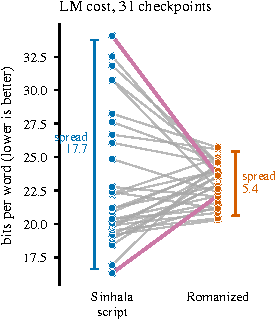
\includegraphics{figures/fig1a_lm_cost.pdf}%
  \caption{}\label{fig:flat-lm}%
\end{subfigure}\hfill%
\begin{subfigure}[b]{0.285\textwidth}%
  \centering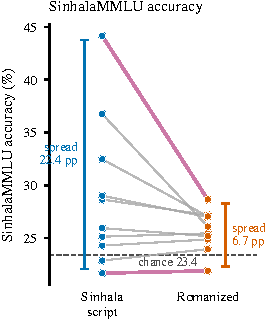
\includegraphics{figures/fig1b_mmlu_accuracy.pdf}%
  \caption{}\label{fig:flat-acc}%
\end{subfigure}\hfill%
\begin{subfigure}[b]{0.345\textwidth}%
  \centering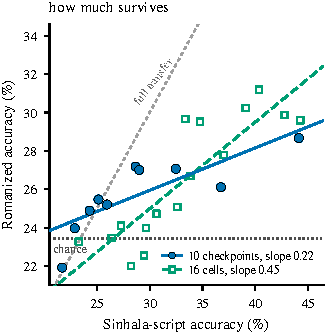
\includegraphics{figures/fig1c_transfer.pdf}%
  \caption{}\label{fig:flat-levels}%
\end{subfigure}
\caption{Romanization narrows the spread between checkpoints.
\subref{fig:flat-lm} Language modeling cost for 31 checkpoints. Word counts are
identical within a pair, so the columns are directly comparable, and the
highlighted lines are checkpoints cheaper on Romanized text.
\subref{fig:flat-acc} SinhalaMMLU accuracy a 22.4 point spread becomes 6.7 and no
checkpoint finishes more than 5.3 points above chance.
\subref{fig:flat-levels} The same numbers as levels, with the 16 domain by
difficulty cells. Both slopes fall well below the full-transfer slope of 1
(bootstrap intervals 0.11 to 0.54 and 0.36 to 0.63). LaMini-GPT-1.5B is omitted
from \subref{fig:flat-acc} and \subref{fig:flat-levels} for unparseable output on
95.9\% of Sinhala-script items.}
\label{fig:flat}
\end{figure*}

\begin{table*}[t]
\centering\footnotesize
\renewcommand{\arraystretch}{0.94}
\setlength{\tabcolsep}{4.6pt}
\begin{tabular}{@{}l r @{\hspace{11pt}} rr @{\hspace{6pt}} r l r @{\hspace{13pt}} rr @{\hspace{6pt}} rr r@{}}
\toprule
& & \multicolumn{5}{c}{\textbf{SinhalaMMLU} (6{,}879 items)}
& \multicolumn{5}{c}{\textbf{SOLD} (2{,}500 items)} \\
\cmidrule(lr){3-7}\cmidrule(lr){8-12}
& & \multicolumn{2}{c}{Accuracy \%}
& \multicolumn{3}{c}{Sinh.\ $-$ Rom.}
& \multicolumn{2}{c}{macro-F1 \%}
& \multicolumn{3}{c}{\mcc} \\
\cmidrule(lr){3-4}\cmidrule(lr){5-7}\cmidrule(lr){8-9}\cmidrule(lr){10-12}
\textbf{Checkpoint} & \textbf{B}
& Sinh. & Rom. & $\Delta$ & 95\% CI & $p_{\text{Holm}}$
& Sinh. & Rom. & Sinh. & Rom. & $p_{\text{Holm}}$ \\
\midrule
\rows{tables/tab_extrinsic_main.tex}
\bottomrule
\end{tabular}
\caption{Downstream results, ordered by size. ``Sinh.'' is the Sinhala-script
condition and ``Rom.'' the Romanized one. For SinhalaMMLU the three grouped columns
describe the paired accuracy difference: $\Delta$ in points, its bootstrap interval,
and McNemar's test corrected across checkpoints within the task. For SOLD the
corrected $p$ belongs to the change in Matthews correlation ($\mcc$), tested by
paired bootstrap. Macro-F1 is reported for reference and is not tested. $\dagger$
marks checkpoints passing the competence screen (\S\ref{sec:screen}). Global PIQA
and the remaining columns are in Appendix~\ref{sec:extradetail}.}
\label{tab:main}
\end{table*}

\subsection{Transfer between the two scripts}
\label{sec:law}

The natural way to state the relationship is that the loss grows with the headroom a
checkpoint had, but that cannot be tested as it stands. Writing headroom as
Sinhala-script accuracy minus chance, a fit across the ten parseable checkpoints gives
$\text{loss} = 0.78 \times \text{headroom} - 1.06$ with $R^2 = 0.96$. Sinhala-script
accuracy is on both axes, so shuffling the Romanized scores to destroy any association
still returns a mean slope of 1.00 and a mean $R^2$ of 0.94, with 8.9\% of permutations
reaching $R^2 \geq 0.96$. We do not treat that fit as evidence.

Stated as levels the same measurements do carry information. Regressing Romanized on
Sinhala-script accuracy gives a slope of 0.22 (95\% bootstrap CI 0.11 to 0.54,
leave-one-checkpoint-out 0.17 to 0.26, $R^2 = 0.65$), below the 1.0 of full transfer
($p = 8.6 \times 10^{-7}$) and above the 0.0 of complete narrowing, since only 0.5\% of
permutations reach the observed fit. Romanization removes roughly four fifths of a
checkpoint's Sinhala-script advantage, and the leave-one-out range shows this is not
driven by one or two points.

Ten checkpoints is a small sample, so we test the same relation inside the benchmark,
with items rather than models as units. Splitting SinhalaMMLU into its 16 non-empty domain
by difficulty cells and pooling the competent cohort within each gives a slope of 0.45
(95\% CI 0.36 to 0.63, leave-one-cell-out 0.43 to 0.50, $R^2 = 0.75$), again below 1.0 at
$p = 1.5 \times 10^{-6}$. The two views aggregate the same generations, so they are not
independent, but they agree on the shape and differ on the magnitude, with content-level
transfer about twice model-level transfer (Appendix Table~\ref{tab:flatten}).

The strata agree (Appendix Table~\ref{tab:strata}). Loss falls monotonically with
difficulty, 7.9 points on Easy items, 6.2 on Medium and 4.3 on Hard, with a significant
interaction in the item-clustered logistic fit ($p < 0.001$), because models sit nearer
chance on hard items in both conditions. By domain it runs from 10.3 points on Social
Science, where Sinhala-script accuracy is highest, to 4.1 on Humanities, the largest
domain. Slices where the models are weaker to begin with reveal smaller script effects.

\subsection{Offensive language detection}

On SOLD the choice of metric changes the conclusion. Accuracy falls by 1.6 to 11.3
points against a 59.4\% majority baseline, a modest change. Matthews correlation gives a
different picture (Appendix Figure~\ref{fig:floor}): Qwen3.5-9B goes from 0.280 to 0.069,
keeping 24\% of its signal, Qwen2-7B-Instruct from 0.148 to 0.042, keeping 29\%, and
Llama-3.1-8B-Instruct from 0.259 to 0.105, keeping 40\%. Five of the six checkpoints with
a real Sinhala-script signal lose significantly under Holm correction and the median keeps
45\%. They drift toward trivial behavior instead. Qwen2-7B-Instruct more than doubles its
rate of predicting the offensive class, 10.5\% to 23.4\%, without becoming more accurate.
A deployment monitored on accuracy alone would see a few points of movement while over
half the usable signal was lost.

\subsection{Global PIQA}
\label{sec:piqa}

These numbers come from a second run, with an instruction that names \textit{Sri Lankan
Culture} and follows each item's form, since the first asked every item for a completion
and 40 of the 100 are questions (Appendix~\ref{sec:prompts}). Sinhala-script accuracy
moves 2.0 points on average. No checkpoint exceeds chance natively, the best being 58\% at
$p = 0.06$, consistent with the 49.09\% that \citet{desilva-ranathunga-2026-sinhalapiqa}
report for SinBERT, and the script comparison is a null. Of the ten checkpoints with
parseable output, four drop, four improve and two are unchanged, a sign test gives
$p = 1.00$ and pooling gives $-0.1$ points (95\% CI $-3.6$ to $+3.3$). At the median of 36
discordant pairs, McNemar's test reaches 80\% power only against a 17.3 point gap, against
1.74 points on SinhalaMMLU's 6{,}879 (Appendix~\ref{sec:extradetail}), so the limit is the
item count
against our effect size rather than anything about the benchmark\nds{The stated purpose of PIQA is to work as a benchmark. Not as a test set.}\stu{Yes sir. We removed the word ``underpowered'' as it is not suitable. Global PIQA works well for its intended purpose of ranking and comparing different models. What we measure is the small drop within the same model when the script changes, and with 100 items a paired test can only resolve much larger effects. We now give the numbers for this in Section~\ref{sec:piqa} instead of using an adjective, and we kept all Global PIQA results in Table~\ref{tab:piqa}. We also re-ran this benchmark with the corrected prompt you pointed out, and with the item types handled properly the gap is now essentially zero rather than a weak trend.}.

\subsection{Two mechanisms ruled out}
\label{sec:controls}

Two competing explanations can be ruled out. The first is token fragmentation, but
romanization does not lengthen Sinhala input. The script costs a median 9.5 tokens per word
against 2.09 for its romanization, because these tokenizers largely fall back to bytes, and
all eleven checkpoints receive \emph{fewer} tokens in the Romanized condition on all three
tasks, a median ratio of 0.48 on SinhalaMMLU. They get shorter input and still do worse.
Splitting items into terciles by token inflation yields no monotone pattern, with losses
of 5.1, 6.6 and 6.2 points. Thin pretraining coverage of Romanized Sinhala would produce this
pattern, and one checkpoint gives partial support (Appendix~\ref{sec:extradetail}), but the
corpora are not open to audit.\nds{Try to avoid window words}\stu{Fixed sir. We removed the widow words and made the paragraphs flow properly.}

The second is output degeneration, since a model could reach chance by emitting one
constant answer. For the competent cohort the share of answers on the most frequent option
is 37.3\% on the Sinhala script and 39.8\% under romanization (Wilcoxon $p = 0.31$), and
the invalid rate never exceeds 0.03\% in either condition, so the checkpoints keep
distributing answers across the option set and are simply wrong more often
(Appendix~\ref{sec:extradetail}).

\subsection{Intrinsic predictors of the gap}
\label{sec:linkage}

A cheap intrinsic measurement partly substitutes for an expensive downstream one, though
not the obvious one. Over the ten checkpoints measured both ways, absolute Sinhala-script
bits per byte tracks the SinhalaMMLU gap ($\rho = -0.83$, 95\% CI $-1.00$ to $-0.30$) and
the loss of Matthews correlation on SOLD ($\rho = -0.78$, CI $-1.00$ to $-0.36$), while
the bits-per-byte \emph{gap}, the counterpart of the ratio
\citet{rajapakse-weerasinghe-2026-script} report, shows no association ($\rho = -0.15$),
and nor does the perplexity ratio ($\rho = -0.52$). With ten checkpoints and intervals
reaching $-1.00$ this is exploratory (Appendix~\ref{sec:linkagedetail}).


% =============================================================================
\section{Conclusion}
\label{sec:conclusion}

Re-measuring 31 small checkpoints with a tokenizer-independent metric changes what the
intrinsic evidence says about Sinhala. About half of the reported 312-fold degradation on
Romanized text is the unit of account rather than model behavior, and once it is removed
parameter count does predict Sinhala-script ability. A benchmark reporting perplexity
across model families on a script that tokenizers handle unevenly reports tokenizer
behavior as much as model behavior, and bits per byte costs nothing extra on the same
forward passes. SinLlama is the extreme case, with the smallest reported degradation here
and one of the widest real per-byte gaps.

Downstream, differences that are clear in the Sinhala script largely disappear under
romanization, with two consequences for practice. Script robustness cannot be read off a
group average, since checkpoints at chance contribute a zero gap by construction and the
hardest strata show the smallest effects, so a claim needs a competence screen and a
stated baseline. And because the checkpoints best on the Sinhala script have the most to
lose, selecting on Sinhala-script scores and then serving Romanized users selects for the
largest drop, and since Romanized ability is nearly flat across a 42-fold parameter range,
scale is not the fix.


\label{sec:endofmain}


% =============================================================================
\section*{Limitations}

\paragraph{Scope.} Everything here is Sinhala, zero-shot and greedy, one template,
open checkpoints up to 14.7B. Few-shot prompting, transliterate-then-infer or
Romanized fine-tuning could each narrow the gap by an unmeasured amount, and stronger
proprietary models have more headroom, so \S\ref{sec:law} predicts larger losses
there.

\paragraph{The Romanized items are transliterated.} No human-typed Romanized version
of these benchmarks exists, so the Romanized side of all three is our
transliterator's output\nds{Do you mean to say that you created 755,000 human-romanized items mentioned in \S\ref{sec:QulHum}?}\stu{No sir we didn't. Reworded this to be clear. 
The 755,000 examples come from an existing public dataset (Swa-bhasha). We only used them as a reference to pick the best transliteration tool and make sure our spellings look like real human typing.}. Attestation does not
predict an item's Romanized penalty on SOLD (Spearman $0.02$, $n = 2{,}447$), and our
text is the harder of the two against human typing (\S\ref{sec:translitbias}), so our
gaps are closer to upper than to lower bounds.

\paragraph{Confounds and weaker evidence.} The 31 checkpoints differ in family,
tokenizer, training corpus and instruction tuning at once, so the parameter-count
association is not a scaling law, and unauditable corpora leave contamination
possible. The intrinsic-to-downstream link rests on ten checkpoints with intervals
reaching $-1.00$ (\S\ref{sec:linkage}); the mixed-script corpus is not parallel to
either condition and two checkpoints cannot follow the format in the Sinhala script,
so their apparent gains are artifacts (\S\ref{sec:screen}).

% \section*{Acknowledgments}

% Omitted for anonymous review. This project uses the universal romanizer software
% `uroman' written by Ulf Hermjakob, USC Information Sciences Institute
% (2015-2020), as required by its license.-

% The two anthology shards are the ACL Anthology's own consolidated BibTeX,
% downloaded from https://aclanthology.org/anthology-1.bib and -2.bib. Keep this
% order: shard 2 uses the @string{anth} that only shard 1 defines. Entries the
% Anthology supplies are cited by its keys and are deliberately absent from
% custom.bib, so nothing is defined twice.
\bibliography{custom,anthology-1,anthology-2}

% =============================================================================
\appendix

\nds{No background on Sinhala provided in the main body or even in the Appendix.}\stu{Added as Appendix~\ref{sec:sinhala}}

\section{Sinhala and its Romanized Register}
\label{sec:sinhala}

\paragraph{The language.} Sinhala (\sisinhala{}) is an Indo-Aryan language and, with
Tamil, an official language of Sri Lanka. It is spoken by more than 17 million people,
almost all of them on the island \citep{desilva-2019-survey,
ranasinghe-etal-2025-sold}. Under the taxonomy of \citet{joshi-etal-2020-state} as
applied by \citet{ranathunga-de-silva-2022-languages} it is low resource, and it is
geographically separated from the South Asian mainland, so it is often left out of
Indic data and model efforts that cover its relatives
\citep{desilva-ranathunga-2026-sinhalapiqa}. Like several South Asian languages it is
diglossic. The written variety and the spoken variety differ in morphology, and
benchmark text is written in the former.

\paragraph{The script.} Sinhala has its own Brahmi-derived script, encoded in
Unicode at U+0D80 to U+0DFF. It is an abugida rather than an alphabet, which is the
property that matters for everything in this paper. A consonant letter already carries
an inherent vowel, so \sika{} is read \rom{ka} and not \rom{k}. To write a different
vowel, a sign is attached to the consonant, giving \sikaa{} for \rom{kaa}; to remove
the vowel, a separate suppression sign, the \textit{hal kirīma}, is attached, giving
\sikhal{} for \rom{k}. One written unit is therefore several code points, and joined
consonant clusters add a zero-width joiner on top of that, so grapheme-level and
code-point-level counts come apart \citep{nisfer2026grapheme}. In UTF-8 each of these
code points costs three bytes, and our corpus averages 2.65 bytes per character against
1.00 for Latin. A tokenizer with no Sinhala pieces in its vocabulary has to fall back to
those bytes, which is where the fertility of 4.3 to 14.2 tokens per word in
Table~\ref{tab:modelids} comes from, and why perplexity on Sinhala is so sensitive to
which tokenizer produced it \citep{velayuthan-sarveswaran-2025-egalitarian}.

\paragraph{The Romanized register.} Formal Sinhala is written in the script, but
informal writing online is dominated by Romanized Sinhala in Latin letters, called
\textit{Singlish} in Sri Lanka. It has no standard orthography and no institutional
one is likely, since it exists precisely to be typed quickly on keyboards laid out for
English. Writers transcribe by ear, so the same word appears many ways. The Swa-bhasha
lexicon records an average of 15.7 accepted Romanized spellings per Sinhala word
\citep{sumanathilaka-etal-2025-swabhasha}, and \sikohomada{} (``how are you'') is typed
\rom{kohomada}, \rom{kohomd} or \rom{kohomade}. The variation is not random. It comes
from vowel length being dropped, from vowels being left out altogether in short function
words, and from English loanwords keeping their English spelling rather than their
Sinhala pronunciation (Table~\ref{tab:mismatch}). Existing Sinhala tooling mostly
converts Latin into Sinhala rather than the reverse
\citep{de-mel-etal-2025-sinhala, sumanathilaka-etal-2025-swabhasha}, on the assumption
that the script is the target form. This paper takes the opposite view for evaluation.
If most input arrives in the Latin-script register, then that is a condition models
should be measured in.


\section{Prompt Templates}
\label{sec:prompts}

One template, T1 below, is used for every dataset and both script conditions. T2
and T3 were the pilot alternatives (\S\ref{sec:prompting}) and are given in full here.
\texttt{\{n\}} is the item's option count and \texttt{\{domain\}}
is the domain name where the dataset provides one.

Every instruction is in English while the item is in Sinhala, in both script
conditions.\nds{What if they ask why the instruction is not in Sinhala}\stu{We have now added three reasons here to cover this. See below.
We also noted in the text that this is a limitation for real world realism.} That is deliberate. The instruction is the part of the prompt that
must not vary, and a Sinhala-script instruction would have to be romanized along with
the item in the Romanized condition, so the wrapper would change at the same time as the
manipulation. English instructions with target-language content are also the usual
setting for zero-shot multilingual evaluation, including in \citet{aravinda2025sinllama}.
The cost is that the setting is less realistic than a fully Sinhala interface would be.

\paragraph{T1, direct (used for every result in this paper).}
\begin{quote}\small\ttfamily
This is a multiple-choice question related to the \{domain\}. Choose the correct
or most appropriate answer from answers 1/.../\{n\} for the following question.
Do not repeat the question or text in your response. Respond with only the number
(1/.../\{n\}) and nothing else.\\
Question: \{question\}\\
1. \{option 1\} ... \{n\}. \{option n\}\\
Answer:
\end{quote}
Global PIQA needs two forms of T1, because its items do.\nds{This is wrong on two accounts: (1) The domain should have been \textit{Sri Lankan Culture}, (2) Not all examples are \textit{complete the text} type. You'd have known this if you actually read the paper and looked at Table 1.}\stu{You were right on both counts sir, and we re-ran the benchmark rather than only fixing the wording. Of the 110 items in your Table 1, 67 are completions and 43 are question and answer pairs, so ``complete the given text'' was wrong for the questions, and the domain should have been \textit{Sri Lankan Culture}. All 11 checkpoints were re-run with the two forms below, and \S\ref{sec:piqa} now reports that run. Sinhala-script accuracy moves by 2.0 points on average and the script gap becomes essentially zero, so the earlier weak trend was partly the prompt. We have kept the earlier numbers in the comparison so the change is visible.}
The released set contains 40 questions and 60 paragraph stems, which is the 43 and 67 of
\citet{desilva-ranathunga-2026-sinhalapiqa} less the ten items the public release omits.
The two are told apart by whether the Sinhala stem ends in a question mark, which agrees
with the \texttt{isQnA} flag recorded for every item. Questions take the same form as
SinhalaMMLU, with \textit{Sri Lankan Culture} as the domain:
\begin{quote}\small\ttfamily
This is a multiple-choice question related to the Sri Lankan Culture. Choose the
correct or most appropriate answer from answers 1/2. Do not repeat the question or
text in your response. Respond with only the number (1/2) and nothing else.\\
Question: \{prompt\}\\
1. \{solution 1\} 2. \{solution 2\}\\
Answer:
\end{quote}
and stems take the completion form, with the domain still named:
\begin{quote}\small\ttfamily
This is related to the Sri Lankan Culture. Out of the given 2 answers, which one is
the best option to complete the given text? Do not repeat the question or text in
your response. Respond with only the number (1/2) and nothing else.\\
\{prompt\}\\
1. \{solution 1\} 2. \{solution 2\}\\
Answer:
\end{quote}
The first run of Global PIQA used the completion wording for every item and left the domain
empty, which fits the 60 stems and not the 40 questions. The prompt pilot of
\S\ref{sec:prompting} used that earlier wording too, so its Global PIQA figure is not
comparable with the run reported in \S\ref{sec:piqa}. Both instructions are
byte-identical across the two script conditions of an item, so in either run the wording
enters the paired difference as a constant; what it can change is the absolute level, which
is why the re-run matters and why we do not interpret that level (\S\ref{sec:piqa}).

Binary classification:
\begin{quote}\small\ttfamily
Classify the following Sinhala text as either 'NOT' (not offensive) or 'OFF'
(offensive). Do not repeat the question or text in your response. Respond with
only 'NOT' or 'OFF' and nothing else.\\
Text: \{text\}\\
Answer:
\end{quote}

\paragraph{T2, two-shot.} The instruction of T1 with ``exactly like the examples
below'' appended, then two fixed exemplars, then the item. The exemplars were written
separately for the pilot and appear in no evaluation set. In full, for a four-option
SinhalaMMLU item in the Romanized condition:\nds{better give an example of the examples}\stu{Added sir.}
\begin{quote}\small\ttfamily
This is a multiple-choice question related to the \{domain\}. Choose the correct or
most appropriate answer from answers 1/2/3/4 for the following question. Do not repeat
the question or text in your response. Respond with only the number (1/2/3/4) and
nothing else, exactly like the examples below.\\[2pt]
Question: lookayee wishaalathama mahaadwiipaya kumakda?\\
1. aasiyaawa 2. aprikaawa 3. yuroopaya 4. oostreeliyaawa\\
Answer: 1\\[2pt]
Question: dinakata paeya kiiyak thibeeda?\\
1. 12 2. 24 3. 48 4. 60\\
Answer: 2\\[2pt]
Question: \{question\}\\
1. \{option 1\} ... \{n\}. \{option n\}\\
Answer:
\end{quote}
The Sinhala-script condition uses the same two questions and options written in the
Sinhala script, with the same answer digits, so the exemplars are paired exactly as the
evaluation items are. Glossed, the two are ``What is the largest continent in the
world?'' with the options Asia, Africa, Europe and Australia, and ``How many hours are
there in a day?'' with 12, 24, 48 and 60. The Global PIQA exemplars are two
two-option physical-commonsense items written the same way, and the SOLD exemplars are
one \texttt{NOT} and one \texttt{OFF} post. All are in the released code.

\paragraph{T3, answer first.} T1 with the response instruction replaced, in full:
\begin{quote}\small\ttfamily
This is a multiple-choice question related to the \{domain\}. Choose the correct or
most appropriate answer from answers 1/.../\{n\} for the following question. Do not
repeat the question or text in your response. State the answer number (1/.../\{n\})
FIRST, before any explanation. You may briefly explain your reasoning only after
giving the number.\\
Question: \{question\}\\
1. \{option 1\} ... \{n\}. \{option n\}\\
Answer:
\end{quote}
Binary classification:
\begin{quote}\small\ttfamily
Classify the following Sinhala text as either 'NOT' (not offensive) or 'OFF'
(offensive). Do not repeat the question or text in your response. State 'NOT' or 'OFF'
FIRST, before any explanation. You may briefly explain your reasoning only after
giving the label.\\
Text: \{text\}\\
Answer:
\end{quote}
\nds{This is the appendix. There are no limits. What stops you from giving the explicit prompt here instead of this replace this part business?}\stu{Fixed sir. T2 and T3 are now
written out in full (including the two exemplars in both script conditions)}
Prompts are rendered through each checkpoint's own chat template. For checkpoints
that emit reasoning traces by default, we disable that behavior identically in
both script conditions. Decoding is greedy at temperature 0 with at most 40 new
tokens, and inputs truncated at 4{,}096 tokens.

\begin{table}[t]
\centering\small
\setlength{\tabcolsep}{3.2pt}
\begin{tabular}{@{}lrrrrr@{}}
\toprule
& \multicolumn{3}{c}{\textbf{Accuracy \%}} & \multicolumn{2}{c}{\textbf{Invalid \%}} \\
\cmidrule(lr){2-4}\cmidrule(lr){5-6}
\textbf{Template} & S & R & both & S & R \\
\midrule
\rows{tables/tab_pilot.tex}
\bottomrule
\end{tabular}
\caption{The prompt-template pilot: 9 checkpoints, 3 templates, 2 script
conditions, 20 items per dataset, 3{,}240 generations. Accuracy counts
unparseable output as wrong. T1 was applied to all three datasets, although T3
scored higher on SOLD and Global PIQA, so that no dataset gets a different
prompting regime (\S\ref{sec:prompting}). At 20 items per dataset none of these
differences is resolvable, which is why the pilot is treated as a format check. Accuracy
is not comparable across the three blocks: chance is 23.4\% on SinhalaMMLU, 50\% on SOLD
and 50\% on Global PIQA, so T1's 44.7\% on Global PIQA is below its baseline while 26.7\%
on SinhalaMMLU is above its own. These Global PIQA numbers use the earlier instruction, not
the corrected one of \S\ref{sec:piqa}.\protect\nds{So by raw accuracy you do better at PIQA than MMLU; but you reject PIQA because it does not meet the stat test?}\protect\stu{Actually sir the raw numbers are misleading because the guessing baselines are different. 
Global PIQA only has 2 choices, so random guessing gives 50\% meaning 44.7\% is worse than flipping a coin. 
SinhalaMMLU has 4 to 5 choices, so guessing gives 23.4\% meaning 26.7\% is actually beating chance. Updated the caption to make this clear too. Also we didn't throw out PIQA sir. All 11 models are fully reported in Table~\ref{tab:piqa}. 
We just don't claim a proven script penalty from it, because 100 questions is too small to tell if a 3 point gap is real or just random sir.}}
\label{tab:pilot}
\end{table}

\section{Checkpoints}
\label{sec:models}

Table~\ref{tab:modelids} lists all 31 checkpoints with their Hugging Face
identifiers and their tokenizer fertility on the parallel corpus. Note the
consistency of Romanized fertility, between 1.9 and 2.4 tokens per word, against
a range of 4.3 to 14.2 on the Sinhala script.

\begin{table*}[t]
\centering\small
\setlength{\tabcolsep}{5pt}
\begin{tabular}{@{}lrlrr@{}}
\toprule
& & & \multicolumn{2}{c}{\textbf{tokens / word}} \\
\cmidrule(lr){4-5}
\textbf{Checkpoint} & \textbf{B params} & \textbf{Hugging Face identifier}
& Sinhala & Romanized \\
\midrule
\rows{tables/tab_model_ids.tex}
\bottomrule
\end{tabular}
\caption{All evaluated checkpoints, with Hugging Face identifiers and tokenizer
fertility on the parallel corpus. $\ddagger$ marks the eleven used for the
downstream evaluation and $\bullet$ the 24 that
\citet{rajapakse-weerasinghe-2026-script} evaluated. Sinhala-script fertility
varies by more than a factor of three across tokenizers, whereas Romanized
fertility is nearly constant.}
\label{tab:modelids}
\end{table*}

\section{Reproducing the Published Benchmark}
\label{sec:repro24}

Table~\ref{tab:shared24} sets our recomputation beside every headline number of
\citet{rajapakse-weerasinghe-2026-script}, on exactly the 24 checkpoints they
evaluated. The agreement is close but not exact. Our median degradation ratio is 312.3
against their published 312.3, and per-checkpoint perplexities agree to a median
absolute difference of 0.05\% on Sinhala script text and 0.004\% on Romanized text, with
a worst case of 0.55\% and 2.01\%. Two mixed script
values, for Phi-4-14B and Mistral-Nemo-Base-2407, differ by more than 5\% and they are
the only points where we cannot reproduce their run. After excluding those two, the
mixed script median difference is 0.39\%. Our conclusions differ from
theirs because of the metric, not because of the measurement.

The two parameter-count correlations flip sign between the two runs, from $+0.09$
to $-0.05$ and from $-0.09$ to $+0.11$. Both are within noise of zero on 24
points and neither is significant in either run, so the reproduction agrees on
what matters, which is that perplexity gives no signal on scale.

\begin{table}[t]
\centering\scriptsize
\setlength{\tabcolsep}{2.4pt}
\begin{tabular}{@{}lrr@{}}
\toprule
\textbf{Quantity} & \textbf{Published} & \textbf{Ours} \\
\midrule
\rows{tables/tab_shared24.tex}
\bottomrule
\end{tabular}
\caption{Our recomputation against the published benchmark, on its own 24
checkpoints. Deviations are per-checkpoint absolute percentage differences from
the published perplexities.}
\label{tab:shared24}
\end{table}

\begin{table*}[t]
\centering\scriptsize
\setlength{\tabcolsep}{5pt}
\begin{tabular}{@{}lr r rr rr r@{}}
\toprule
& & & \multicolumn{2}{c}{\textbf{token-count normalizer}}
& \multicolumn{2}{c}{\textbf{per-byte loss}} & \\
\cmidrule(lr){4-5}\cmidrule(lr){6-7}
\textbf{Checkpoint} & \textbf{ratio} & \textbf{bits} & bits & factor & bits & factor
& \textbf{norm.\ \%} \\
\midrule
\rows{tables/tab_decomp.tex}
\bottomrule
\end{tabular}
\caption{Equation~\ref{eq:decomp} applied to every checkpoint, sorted by the
reported perplexity ratio. ``ratio'' is Romanized over Sinhala-script perplexity
and ``bits'' its base-2 logarithm, which the two terms partition exactly. The
last column is the normalizer's share of the total. $\bullet$ marks the 24
checkpoints of \citet{rajapakse-weerasinghe-2026-script}. For the Qwen3.5 and Gemma checkpoints the
normalizer term is slightly negative, because their tokenizers spend about the
same number of bytes per token in both scripts, and those are also the
checkpoints with the smallest reported ratios.}
\label{tab:decomp}
\end{table*}

\section{The Sinhala Adapted Checkpoint}
\label{sec:sinllamadetail}

Table~\ref{tab:sinllama} supports \S\ref{sec:sinllama}. SinLlama
\citep{aravinda2025sinllama} merges 11{,}080 Sinhala pieces into the Llama-3 vocabulary,
taking it from 128{,}256 to 139{,}336 entries, and continues pre-training on 10.7M
Sinhala sentences drawn from MADLAD-400 and CulturaX. We score the released adapter
merged into its base, and we score \texttt{Meta-Llama-3-8B} itself under the same
protocol, since the pool of 31 contains Llama-3.1-8B and a comparison against that would
confound the Sinhala adaptation with the 3 to 3.1 update. The two Llama versions share a
tokenizer and land within 0.008 bits per byte of each other, so the substitution would
not have been badly wrong, but the exact parent makes the contrast clean.

Three further details are worth recording. First, the decomposition of
Equation~\ref{eq:decomp} stops being informative on this checkpoint. Its tokenizer
spends 9.90 bytes per token on the Sinhala script and 2.77 on Romanized text, so the two
terms come out at $-14.26$ and $+17.38$ bits and sum to the observed 3.11. The identity
still holds exactly, but a ratio that is the residue of two much larger opposing
quantities is not a quantity to interpret, which is itself an argument against reading
the ratio at all. Second, SinLlama was continually pre-trained on web-crawled Sinhala,
and our intrinsic corpus is Sinhala text from the web, so we cannot rule out that some
of these sentences or near-duplicates were in its training data; that would inflate its
Sinhala-script advantage and not its Romanized one, so it does not affect the direction
of the asymmetry. Third, \texttt{meta-llama/Meta-Llama-3-8B} is gated, and our run loaded
the widely used ungated mirror of it. The four \texttt{safetensors} shards carry the same
sizes and SHA-256 digests as the official repository, and the tokenizer reproduces the
recorded Llama-3.1 fertility exactly.

\begin{table}[t]
\centering\scriptsize
\setlength{\tabcolsep}{2.4pt}
\begin{tabular}{@{}l r r rr rr r r@{}}
\toprule
& & \multicolumn{3}{c}{\textbf{Sinhala script}} & \multicolumn{2}{c}{\textbf{Rom.}}
& & \\
\cmidrule(lr){3-5}\cmidrule(lr){6-7}
\textbf{Checkpoint} & \textbf{t/w} & PPL & \bpb{} & \bpw{} & \bpb{} & \bpw{}
& \textbf{ratio} & \boldmath$\Delta\bpb$ \\
\midrule
\rows{tables/tab_sinllama.tex}
\bottomrule
\end{tabular}
\caption{A Sinhala-adapted checkpoint against the exact base model it was built from,
on the same 500 sentence pairs as the pool. ``t/w'' is Sinhala-script tokens per word,
``ratio'' is Romanized over Sinhala-script perplexity, and $\Delta\bpb$ is the real
per-byte gap between the two conditions. The adaptation gives the lowest Sinhala-script
bits per byte and the highest Sinhala-script perplexity of anything we measured, and it
takes the reported ratio from 311 to 8.7 while making the per-byte gap wider.
$^{\dagger}$ is the best of the 31 by Sinhala-script bits per byte, for scale. Neither
of the first two rows is included in the pool of 31.}
\label{tab:sinllama}
\end{table}

\section{Sinhala Tokenizers}
\label{sec:tokenizers}

Table~\ref{tab:tokenizers} measures the Sinhala specific tokenizers of
\S\ref{sec:related} on our parallel corpus. Fertility needs no forward pass, so it can
be reported for encoders too, whose per token likelihoods are not comparable with the
causal checkpoints of Table~\ref{tab:intrinsicfull}. Counts here are subword pieces per
whitespace word with no special tokens, which differs from the recorded runs by at most
one token per sentence, or 0.17 tokens per word, because those count predicted tokens.

The pattern is consistent. A purpose built Sinhala vocabulary reduces Sinhala-script
fertility from the 4.34 to 14.20 range of the general tokenizers down to 1.31 or 1.44,
a factor of three to seven. None of them improves the Romanized register and the
Sinhala only vocabulary of SinBERT makes it markedly worse at 6.15 tokens per word,
since Latin text has to be assembled from pieces chosen for the Sinhala script.
HelaBERT's unigram model also emits a separate whitespace piece before each Latin word,
which accounts for about half of its Romanized count. Tokenizer work for Sinhala is
therefore effective on the script it targets and leaves the Latin-script register where
it was.

\begin{table}[t]
\centering\small
\setlength{\tabcolsep}{4pt}
\begin{tabular}{@{}lrcc@{}}
\toprule
& & \multicolumn{2}{c}{\textbf{tokens / word}} \\
\cmidrule(lr){3-4}
\textbf{Tokenizer} & \textbf{vocab} & Sinhala & Romanized \\
\midrule
\rows{tables/tab_tokenizers.tex}
\bottomrule
\end{tabular}
\caption{Tokenizer fertility on the 500 sentence parallel corpus. The first three are
Sinhala specific vocabularies and the last two rows are the 31 general checkpoints of
Table~\ref{tab:modelids}. A Sinhala vocabulary cuts Sinhala-script fertility several
fold and does nothing for the Romanized register, where the Sinhala only vocabulary is
the least efficient of all.}
\label{tab:tokenizers}
\end{table}

\section{Full Intrinsic Results}
\label{sec:fullintrinsic}

Table~\ref{tab:intrinsicfull} gives every metric for every checkpoint in all three
script conditions, corpus-pooled as in Equation~\ref{eq:bpb}.
Table~\ref{tab:ngram} and Figure~\ref{fig:ngram} give the character $n$-gram
reference of \S\ref{sec:intrinsic}.

\begin{table*}[t]
\centering\scriptsize
\setlength{\tabcolsep}{3.4pt}
\begin{tabular}{@{}lr rrrr rrrr rrr@{}}
\toprule
& & \multicolumn{4}{c}{\textbf{Sinhala script}} & \multicolumn{4}{c}{\textbf{Romanized}}
& \multicolumn{3}{c}{\textbf{Mixed script}} \\
\cmidrule(lr){3-6}\cmidrule(lr){7-10}\cmidrule(lr){11-13}
\textbf{Checkpoint} & \textbf{B} & PPL & \bpb{} & \bpc{} & \bpw{}
& PPL & \bpb{} & \bpc{} & \bpw{} & PPL & \bpb{} & \bpw{} \\
\midrule
\rows{tables/tab_intrinsic_full.tex}
\bottomrule
\end{tabular}
\caption{Corpus-pooled intrinsic metrics for all 31 checkpoints in all three script
conditions, sorted by Sinhala-script bits per byte. $\ddagger$ marks the eleven
checkpoints also evaluated downstream. The perplexity and bits-per-byte orderings
disagree almost completely. Gemma-2-9B is 2nd by Sinhala-script bits per byte and 26th
by Sinhala-script perplexity.}
\label{tab:intrinsicfull}
\end{table*}

\begin{table}[t]
\centering\small
\setlength{\tabcolsep}{4pt}
\begin{tabular}{@{}lcccc@{}}
\toprule
& \multicolumn{2}{c}{\textbf{Sinhala script}} & \multicolumn{2}{c}{\textbf{Romanized}} \\
\cmidrule(lr){2-3}\cmidrule(lr){4-5}
\textbf{Model} & \bpb{} & \#\,LMs $<$ & \bpb{} & \#\,LMs $<$ \\
\midrule
\rows{tables/tab_ngram.tex}
\bottomrule
\end{tabular}
\caption{Held-out add-1 character $n$-gram models against the 31 checkpoints,
five-fold cross-validated so every score is out of sample. ``\#\,LMs $<$'' counts
checkpoints that achieve lower bits per byte than the $n$-gram model. No
checkpoint beats a character bigram on Romanized Sinhala.}
\label{tab:ngram}
\end{table}

\begin{figure}[t]
\centering
\begin{subfigure}[b]{\columnwidth}%
  \centering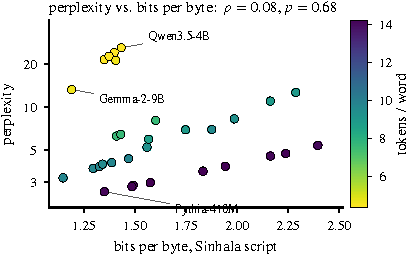
\includegraphics{figures/fig2a_ppl_vs_bpb.pdf}%
  \caption{}\label{fig:ppl-bpb}%
\end{subfigure}

\begin{subfigure}[b]{\columnwidth}%
  \centering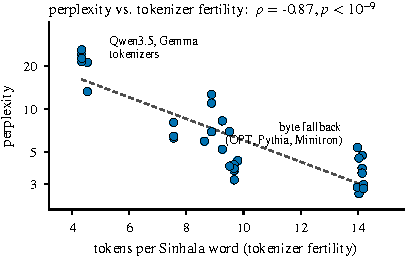
\includegraphics{figures/fig2b_ppl_vs_fertility.pdf}%
  \caption{}\label{fig:ppl-fert}%
\end{subfigure}
\caption{What Sinhala-script perplexity is measuring.
\subref{fig:ppl-bpb} Across 31 checkpoints it is unrelated to Sinhala-script bits
per byte. \subref{fig:ppl-fert} It is instead almost fully determined by how many
tokens the tokenizer spends per Sinhala word.}
\label{fig:ppl}
\end{figure}

\begin{figure}[t]
\centering
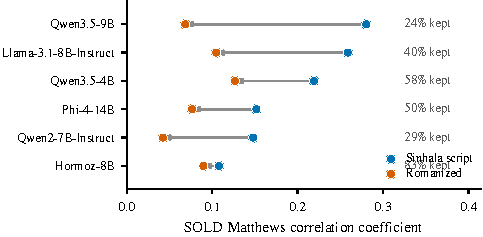
\includegraphics[width=\columnwidth]{figures/fig3_sold_mcc.pdf}
\caption{Matthews correlation on SOLD for the six checkpoints with a real
Sinhala-script signal, with the percentage retained under Romanization. Accuracy
for the same checkpoints moves by only 1.6 to 11.3 points
(Table~\ref{tab:main}).}
\label{fig:floor}
\end{figure}

\begin{figure}[t]
\centering
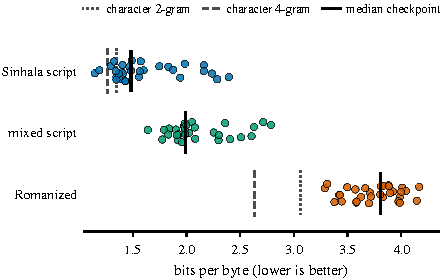
\includegraphics[width=\columnwidth]{figures/fig4_ngram_reference.pdf}
\caption{Bits per byte for all 31 checkpoints in each script condition, with
held-out character $n$-gram references. The mixed-script corpus is not parallel,
so no reference is shown for it.}
\label{fig:ngram}
\end{figure}

\begin{figure}[t]
\centering
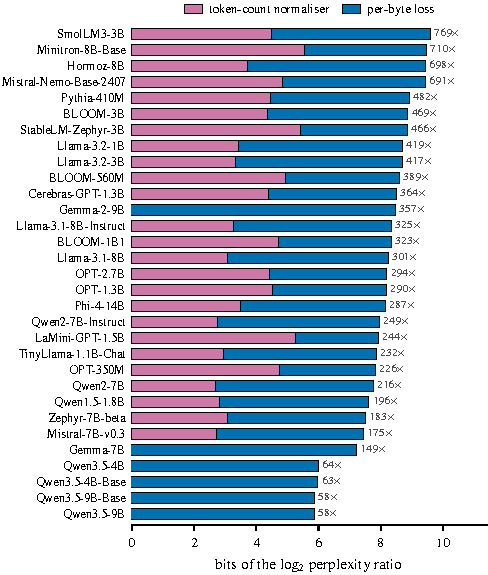
\includegraphics[width=\columnwidth]{figures/fig5_ppl_decomposition.pdf}
\caption{Where the reported degradation ratio comes from, per checkpoint. Each bar
is the base-2 logarithm of that checkpoint's perplexity ratio, split exactly by
Equation~\ref{eq:decomp} into the part caused by identical content occupying a
different number of tokens and the part caused by a real rise in per-byte loss.
The annotation is the raw ratio. The six checkpoints with no visible normalizer
term are the Qwen3.5 and Gemma models, whose tokenizers are efficient on the
Sinhala script.}
\label{fig:decomp}
\end{figure}




\section{Additional Downstream Detail}
\label{sec:extradetail}

Table~\ref{tab:invalidtau} gives the unparseable-output rates and the input token
ratios omitted from Table~\ref{tab:main}, Table~\ref{tab:strata} the SinhalaMMLU
strata, and Table~\ref{tab:piqa} the per-checkpoint Global PIQA results.

Two splits of Global PIQA are worth recording, since neither rescues a script effect
from it. Pooled over the ten parseable checkpoints, the 40 question items give
$+1.0$ points and the 60 paragraph stems $-0.8$, so the item form the instruction now
distinguishes does not carry the comparison. The 77 items flagged culturally specific
give $+1.2$ points and the remaining 23 give $-4.3$, both far inside what 100 items can
resolve. Unparseable output is rare in this run: zero for eight of the eleven
checkpoints in both conditions, at most 9\% for TinyLlama-1.1B-Chat, and 100\% in the
Sinhala script for LaMini-GPT-1.5B. Only that checkpoint survives Holm correction, and
its apparent 42 point gain is the same parsing artifact (\S\ref{sec:screen}).

The power figures behind \S\ref{sec:piqa} are these. Against the 6.0 point gap we pool on
SinhalaMMLU, McNemar's test on 36 discordant pairs has power 0.13, and reaching 80\% power
for that gap would need about 825 items. Comparing the two runs, Sinhala-script accuracy
differs by 2.0 points on average and rises for five of the eleven checkpoints, while the
number of checkpoints scoring lower on Romanized text falls from seven to four, so the
corrected instruction moves the absolute level and removes the weak downward trend the
first run showed.

One checkpoint lets us check the pretraining-exposure reading of
\S\ref{sec:controls} directly. BLOOM's corpus covers 46 languages and Sinhala is not
one of them \citep{laurencon-etal-2023-roots, lescao-etal-2023-bloom}, and all three
BLOOM checkpoints sit at or near the bottom of Table~\ref{tab:intrinsicfull} on
Sinhala-script text while being unremarkable on Romanized text. Exposure is
documented for no other checkpoint in the pool.

\begin{table}[t]
\centering\small
\setlength{\tabcolsep}{4pt}
\begin{tabular}{@{}lrrrrr@{}}
\toprule
\textbf{Stratum} & \textbf{Items} & \textbf{S \%} & \textbf{R \%}
& \boldmath$\Delta$ & \boldmath$p_{\text{Holm}}$ \\
\midrule
\rows{tables/tab_strata.tex}
\bottomrule
\end{tabular}
\caption{SinhalaMMLU by stratum, pooled over the six competent checkpoints. Item
counts are per checkpoint. Domains are ordered by loss.}
\label{tab:strata}
\end{table}

\begin{table}[t]
\centering\small
\setlength{\tabcolsep}{2.2pt}
\begin{tabular}{@{}lrrrrr@{}}
\toprule
& \multicolumn{2}{c}{\textbf{MMLU inv.\ \%}} & \multicolumn{2}{c}{\textbf{PIQA inv.\ \%}} & \\
\cmidrule(lr){2-3}\cmidrule(lr){4-5}
\textbf{Checkpoint} & S & R & S & R & \boldmath$\tau$ \\
\midrule
\rows{tables/tab_invalid_tau.tex}
\bottomrule
\end{tabular}
\caption{Unparseable-output rates, and $\tau$, the ratio of Romanized to
Sinhala-script input tokens on SinhalaMMLU. $\tau$ is below one for every
checkpoint, so the Romanized condition is the shorter input in every case.}
\label{tab:invalidtau}
\end{table}

\begin{table}[t]
\centering\small
\setlength{\tabcolsep}{3.4pt}
\begin{tabular}{@{}lrrrcr@{}}
\toprule
& \multicolumn{2}{c}{Acc.\ \%} & & \textbf{disc.} & \\
\cmidrule(lr){2-3}\cmidrule(lr){5-5}
\textbf{Checkpoint} & S & R & \boldmath$\Delta$ & \textbf{b/c}
& \boldmath$p_{\text{Holm}}$ \\
\midrule
\rows{tables/tab_piqa.tex}
\bottomrule
\end{tabular}
\caption{Global PIQA, 100 items, from the re-run with the item-type-aware
instruction of Appendix~\ref{sec:prompts}. ``disc.\ b/c'' are the discordant pair
counts entering McNemar's test. No checkpoint is above chance in the Sinhala-script
condition, and the only comparison surviving correction is LaMini-GPT-1.5B, which
cannot produce a parseable answer in the Sinhala script at all, so its 42 point
``gain'' is an artifact (\S\ref{sec:screen}). With 100 items this task neither
supports nor contradicts the effect measured on the other two (\S\ref{sec:piqa}).}
\label{tab:piqa}
\end{table}

\begin{table}[t]
\centering\scriptsize
\setlength{\tabcolsep}{2pt}
\begin{tabular}{@{}lr@{}}
\toprule
\textbf{Fit} & \textbf{Value} \\
\midrule
\rows{tables/tab_flatten.tex}
\bottomrule
\end{tabular}
\caption{Every refit of the two transfer regressions of \S\ref{sec:law}. The
levels form regresses Romanized on Sinhala-script accuracy. The headroom form
regresses the paired loss on Sinhala-script headroom above chance, and is reported
only to show why we do not rely on it under a permutation null that destroys any
association between the two conditions, it still returns a mean slope of 1.00 and
a mean $R^2$ of 0.94, because Sinhala-script accuracy appears on both axes. The
levels form returns a mean slope of 0.00 and a mean $R^2$ of 0.11 under the same
null.}
\label{tab:flatten}
\end{table}


\section{The Transliterator}
\label{sec:translitdetail}

\subsection{Quality against human references}
\label{sec:QulHum}

Table~\ref{tab:methods} compares our method with Aksharamukha
\citep{rajan-aksharamukha}, uroman \citep{hermjakob-etal-2018-box} and the web
romanizer released for \citet{desilva-ranathunga-2026-sinhalapiqa}, against
755{,}000 human-romanized items. Ours has the lowest character error rate on all
three corpora. The web tool comes close once its \rom{v} is rewritten to \rom{w},
which is a spelling convention rather than a transliteration error, but it cannot
romanize 17 sequences involving \sinya{} at all and leaves Sinhala characters in
0.8\% to 2.5\% of its output.

\begin{table}[t]
\centering\small
\setlength{\tabcolsep}{2.2pt}
\begin{tabular}{@{}lccccc c@{}}
\toprule
& \multicolumn{3}{c}{\textbf{CER} $\downarrow$} & \textbf{chrF} & \textbf{Exact} & \textbf{Cov.} \\
\cmidrule(lr){2-4}\cmidrule(lr){5-5}\cmidrule(lr){6-6}\cmidrule(lr){7-7}
\textbf{Method} & sent. & word & aug. & sent. & word & \% \\
\midrule
\rows{tables/tab_methods.tex}
\bottomrule
\end{tabular}
\caption{Transliteration quality against human references: 4{,}397 authentic
social-media sentence pairs, 450{,}587 multi-reference words, and a fixed
300{,}000-sentence sample of a machine-augmented set. Coverage is the share of
inputs the method produced any output for.}
\label{tab:methods}
\end{table}

\subsection{How our spellings differ from human typing}

Aligning our output word by word against the human-typed Romanized side of the
parallel corpus, 485 of the 500 sentences have matching token counts, giving
2{,}933 aligned word pairs. Of those, 44.6\% match exactly. A further 27.6\% match
once runs of the same Latin vowel are collapsed, which is the one convention our
transliterator applies uniformly and people apply erratically. The remaining
27.8\% differ in some other way, and Table~\ref{tab:mismatch} lists the most
frequent. They are dominated by vowel reduction and abbreviation: people write
\rom{mn} for our \rom{man} and \rom{dan} for our \rom{daen}. English loanwords are
a smaller but more consequential class, concentrated in the sentences that diverge
most, where a person writes \rom{phone}, \rom{video} or \rom{tv} and our
transliterator renders the Sinhala spelling of the same word as \rom{foon},
\rom{wiidiyoo} or \rom{tiiwii}.

Table~\ref{tab:attest} bounds how much this matters, using the
450{,}587-word Swa-bhasha lexicon, which records every Romanized spelling a human
supplied for each Sinhala word and averages 15.7 accepted spellings per word.
Once the long-vowel convention is normalized, 88.6\% of our word tokens in the
parallel corpus carry a spelling some human actually supplied for that word, and
87.0\% on SOLD. The reference point is the row above. The native speakers who typed
the same 500 sentences match the lexicon 84.2\% of the time by the same measure. Our
spellings are therefore attested about as often as human typing is.

\begin{table}[t]
\centering\footnotesize
\setlength{\tabcolsep}{2.4pt}
\begin{tabular}{@{}lrrrr@{}}
\toprule
& & & \multicolumn{2}{c}{\textbf{attested \%}} \\
\cmidrule(lr){4-5}
\textbf{Text} & \textbf{tokens} & \textbf{cov.\ \%} & raw & norm. \\
\midrule
\rows{tables/tab_attest.tex}
\bottomrule
\end{tabular}
\caption{Share of word tokens whose Romanized spelling is one a human supplied
for that Sinhala word in the Swa-bhasha lexicon. ``tokens'' counts the word
tokens the lexicon covers and ``cov.'' the share of all Sinhala word tokens that
is. ``norm.'' collapses runs of the same Latin vowel on both sides. The first row
is the reference point: it applies the same measure to text native speakers
typed.}
\label{tab:attest}
\end{table}

\begin{table}[t]
\centering\small
\begin{tabular}{@{}llr@{}}
\toprule
\textbf{Ours} & \textbf{Human} & \textbf{n} \\
\midrule
\rows{tables/tab_mismatch.tex}
\bottomrule
\end{tabular}
\caption{The twelve most frequent word-level disagreements with the human-typed
side of the parallel corpus that survive normalizing the long-vowel convention.
Most are vowel reduction or abbreviation on the human side.}
\label{tab:mismatch}
\end{table}

\subsection{What the residual costs a model}
\label{sec:translitbias}

The spelling statistics above establish that our output is plausible Singlish, but
not whether a model finds it easier or harder than the real thing, which is what
decides whether our downstream gaps are over- or under-estimates. The parallel
corpus lets us measure that directly, because it already carries a Romanized side
that native speakers typed for the same 500 sentences. We added a third condition,
our transliterator's output for those sentences, and scored all three with the
protocol of \S\ref{sec:intrinsic}.

Table~\ref{tab:svh} reports six checkpoints, scored on CPU so that the control did
not compete with the main runs for GPU time. The Sinhala-script and human-typed
columns reproduce the recorded run to within 0.11\%, which is an independent check on
the intrinsic pipeline. The quantity of interest is the difference. Our
transliteration costs 0.17 to 0.24 more bits per byte than the human-typed text on
identical content, with the same sign for every checkpoint. Our Romanized condition
is therefore the harder of the two, so the downstream gaps in \S\ref{sec:extrinsic}
are more likely upper bounds than lower bounds.

The same table makes the methodological point of \S\ref{sec:intrinsic} on a smaller
scale. Per-token perplexity is \emph{lower} on our text than on the human text for
every checkpoint, a median ratio of 0.74, because our spellings are longer and
occupy more tokens. Perplexity therefore rates our transliteration as the easier of
the two while bits per byte rates it as the harder one, on identical content.

\begin{table}[t]
\centering\scriptsize
\setlength{\tabcolsep}{2.6pt}
\begin{tabular}{@{}lr rrr rr@{}}
\toprule
& & \multicolumn{3}{c}{\textbf{bits per byte}} & & \textbf{PPL} \\
\cmidrule(lr){3-5}
\textbf{Checkpoint} & \textbf{B} & Sinh. & human & ours
& \boldmath$\Delta$ & ratio \\
\midrule
\rows{tables/tab_svh.tex}
\bottomrule
\end{tabular}
\caption{Our transliteration against human typing on the same 500 sentences.
$\Delta$ is ours minus human bits per byte, positive meaning our text is harder.
``PPL ratio'' is our perplexity over the human perplexity, below one for every
checkpoint even though bits per byte is higher, because our spellings occupy more
tokens. The Sinhala-script and human columns reproduce the recorded run to within
0.11\%. $\ddagger$ marks checkpoints also evaluated downstream. The control was
scored on CPU, which is why it is run over the smaller end of the pool.}
\label{tab:svh}
\end{table}

\begin{table}[t]
\centering\scriptsize
\setlength{\tabcolsep}{2pt}
\begin{tabular}{@{}l r@{~}l r@{~}l@{}}
\toprule
& \multicolumn{2}{c}{\textbf{MMLU gap}} & \multicolumn{2}{c}{\textbf{SOLD} $\Delta\mcc$} \\
\cmidrule(lr){2-3}\cmidrule(lr){4-5}
\textbf{Intrinsic predictor} & $\rho$ & 95\% CI & $\rho$ & 95\% CI \\
\midrule
\rows{tables/tab_linkage.tex}
\bottomrule
\end{tabular}
\caption{Spearman correlations between intrinsic measurements and downstream
script effects, over the ten parseable checkpoints, with bootstrap intervals.
Levels track the effect, gaps and ratios do not. The intervals are wide because
$n = 10$, which is why this is exploratory.}
\label{tab:linkage}
\end{table}

\begin{table}[t]
\centering\small
\setlength{\tabcolsep}{2.8pt}
\begin{tabular}{@{}lrr rrr l@{}}
\toprule
\textbf{Attest.} & \textbf{items} & \textbf{att.\ \%}
& \textbf{S \%} & \textbf{R \%} & \boldmath$\Delta$ & \textbf{95\% CI} \\
\midrule
\rows{tables/tab_attest_tercile.tex}
\bottomrule
\end{tabular}
\caption{SOLD items split into terciles by how often their Romanized spellings are
attested in the human lexicon, pooled over the five competent checkpoints. If our
transliterator's idiosyncrasies drove the Romanized penalty, the low-attestation
tercile would lose most. It loses least, and per item the correlation between
attestation and loss is Spearman $0.02$ ($p = 0.31$, $n = 2{,}447$). The tercile
with the smallest gap also has the lowest Sinhala-script accuracy, which the
narrowing of \S\ref{sec:law} already predicts.}
\label{tab:attesttercile}
\end{table}



\section{Intrinsic Predictors in Detail}
\label{sec:linkagedetail}

This expands \S\ref{sec:linkage}. Table~\ref{tab:linkage} gives every intrinsic
measurement against both downstream script effects, with bootstrap intervals, over the
ten parseable checkpoints.

Absolute Sinhala-script bits per byte tracks the SinhalaMMLU gap ($\rho = -0.83$, 95\% CI
$-1.00$ to $-0.30$, leave-one-out $-0.90$ to $-0.77$) and the loss of Matthews
correlation on SOLD ($\rho = -0.78$, CI $-1.00$ to $-0.36$, leave-one-out $-0.87$ to
$-0.73$). The bits-per-byte \emph{gap} shows no association ($\rho = -0.15$, CI $-0.89$
to $+0.63$) and neither does the perplexity ratio ($\rho = -0.52$). For the gap the
leave-one-out range straddles zero, so we cannot even sign it; with ten checkpoints that
is an absence of evidence rather than evidence of absence.

\nds{Again a paragraph too obviously AI.}\stu{Rewritten}We are not proposing this as a working predictor. There are ten checkpoints, we did not
hold any of them out, and some intervals run to $-1.00$. What survives leave-one-out is
the ordering, that levels carry information here and gaps do not, and that is the part
worth trying on a larger set of checkpoints.


\section{Licenses and Redistribution}
\label{sec:licenses}

\begin{itemize}\itemsep2pt
\item \textbf{SinhalaMMLU} \citep{pramodya-etal-2025-sinhalammlu}: CC BY-NC-ND
4.0, gated. The public release is a 1{,}851-item sample. We obtained the full
6{,}879-item set from the authors by email in August 2026, and they asked that it
not be redistributed. The NoDerivatives term also forbids distributing
adaptations, and our Romanized version is one. We therefore redistribute neither
the items nor their romanization. We release the transliteration and
set-construction code, the item identifiers, and a SHA-256 digest of the frozen
file, so a reader with their own copy of the full set can rebuild ours and confirm
it is byte-identical. The NoDerivatives term applies to the public sample as much as to
the full set, so we cannot ship a Romanized version of that either, but the
set-construction code runs unchanged on the public release, so a reader with only that
can build the Romanized side themselves. Every row of the public sample is labelled
\texttt{difficulty=Easy}, so the difficulty strata of \S\ref{sec:law} are not
reproducible from it. Everyone can reproduce the SOLD and Global PIQA results
in full.
\item \textbf{SOLD} \citep{ranasinghe-etal-2025-sold}: publicly released for
research through its Hugging Face dataset and its repository, neither of which
carries an explicit license file. We redistribute the 2{,}500-item test split with
our Romanized side attached, in the same pseudonymized form as upstream, and will
remove it on request from the authors.
\item \textbf{Global PIQA} \citep{chang-etal-2025-globalpiqa,
desilva-ranathunga-2026-sinhalapiqa} under CC BY-SA 4.0, evaluation only. The authors
forbid training on it or on synthetic data seeded from it. We do no training. Our
Romanized version is a derivative and is redistributed under the same CC BY-SA 4.0
terms.\nds{You need to explain why you are using your romanised version instead of the one provided in the dataset itself}\stu{Added an explanation here sir.}
The release also publishes a \texttt{sin\_latn} config for Sinhala, and we do not use it
as our Romanized condition. It contains the same 100 items, verified by matching all 200
English glosses, but written in a scholarly transliteration with diacritics in the style
of ISO~15919. Only 86.4\% of its characters are ASCII and 61.1\% of its words carry at
least one non-ASCII character, at 1.178 bytes per character against 1.000 for ours.
Three consequences rule it out for this paper. It is not the register we study: Romanized
Sinhala as people type it is plain ASCII on an English keyboard, which is what our
transliterator produces and what the Swa-bhasha references attest
(\S\ref{sec:translitdetail}). Its diacritics and zero-width joiners are rare characters
that tokenizers fragment, so adopting it would reintroduce the byte-and-token confound
the paper exists to remove. And it exists for Global PIQA alone, so using it for one
dataset and our transliterator for the other two would make the script condition mean
something different in each task. It is also registered as its own language in the
release, with its own example identifiers and its own answer ordering, so it is not a
drop-in paired twin.

\item \textbf{Swa-bhasha Resource Hub}
\citep{sumanathilaka-etal-2025-swabhasha} used only to select and validate the
transliterator. We redistribute none of it and our code downloads it from source.
\item \textbf{The parallel and mixed-script intrinsic corpora}
\citep{rajapakse-weerasinghe-2026-script} released publicly with that paper and
redistributed unchanged.
\item \textbf{Aksharamukha} \citep{rajan-aksharamukha} AGPL-3.0, version 2.3,
called as a library for comparison only. \textbf{uroman}
\citep{hermjakob-etal-2018-box} version 1.3.1.1, MIT-style license with a
required acknowledgment, which appears in the Acknowledgments section as its
license directs.
\item \textbf{Model weights}: evaluation only, no fine-tuning and no derivative
release, which is within the terms of the Llama Community License, the Gemma Terms
of Use, the BigScience RAIL license and the Apache-2.0 and MIT licenses covering
the remaining families.
\end{itemize}

\section{Reproducibility and Compute}
\label{sec:repro}

Every number in this paper is produced by scripts that read only the per-item
model outputs, so the tables and figures cannot drift from the data. A checking
script re-derives every figure quoted in the text from the frozen analysis and
fails if any has moved. We release the frozen evaluation sets with both script
conditions paired per record, subject to \S\ref{sec:licenses}, all per-item
generations for every checkpoint, the analysis and figure scripts, and the
transliterator: \anonrepo. The transliterator is also on PyPI, but naming the
package would identify us, so the name is withheld until the camera-ready version.

Intrinsic evaluation scores 46{,}500 sequences, 31 checkpoints at 1{,}500
sequences each. Downstream evaluation produces 208{,}538 generations, 11
checkpoints over 9{,}479 items in two script conditions. Both use fp16. Total
wall-clock time was about 80 hours, roughly 10 hours for the intrinsic runs and 70
for the downstream runs, of which about 25 hours were Phi-4-14B alone. All runs
used commodity dual T4 GPUs except Phi-4-14B, which ran on a single 16\,GB
RTX 4070 Ti SUPER. The transliteration control of \S\ref{sec:translitbias} adds
9{,}000 scored sequences and ran in under an hour on eight CPU cores in fp32,
which is why its reproduction deviations are non-zero.

Greedy decoding and a fixed template make the downstream runs deterministic up to
GPU non-determinism, and the transliteration and data preparation steps are fully
deterministic with byte-identical outputs recorded as SHA-256 digests.


\end{document}
